% ====================================================================
% IEEE Conference Paper — Urdu Prompting Study
% ====================================================================
\documentclass[conference]{IEEEtran}
\IEEEoverridecommandlockouts

\usepackage{cite}
\usepackage{amsmath,amssymb,amsfonts}
\usepackage{algorithmic}
\usepackage{graphicx}
\usepackage{textcomp}
\usepackage{xcolor}
\usepackage{booktabs}
\usepackage{hyperref}
\usepackage{url}
\usepackage{multirow}

\def\BibTeX{{\rm B\kern-.05em{\sc i\kern-.025em b}\kern-.08em
    T\kern-.1667em\lower.7ex\hbox{E}\kern-.125emX}}

\begin{document}

\title{Does Prompting Language Matter for Urdu Sentiment Analysis on Small Multilingual Language Models?}

\author{
\IEEEauthorblockN{Author 1, Author 2, Author 3}
\IEEEauthorblockA{Department of Computer Science\\
FAST National University of Computer and Emerging Sciences, Lahore, Pakistan\\
Email: \{l21XXXX, l21XXXX, l21XXXX\}@lhr.nu.edu.pk}
}

\maketitle

% --------------------------------------------------------------------
\begin{abstract}
Small instruction-tuned language models (sub-2B parameters) have made
prompt-based inference a practical alternative to full fine-tuning for
downstream NLP tasks, yet their behaviour on low-resource, non-Latin-script
languages such as Urdu is poorly understood. A specific open question is
whether prompts written in the target language (Urdu) or in English---the
language that dominates the instruction-tuning mix---yield better task
performance. We conduct a systematic comparison of English and Urdu prompts
across two small multilingual instruct models (Qwen2.5-0.5B, Qwen2.5-1.5B)
and three prompting regimes (zero-shot, 3-shot, chain-of-thought) on the
task of ternary Roman-Urdu sentiment classification, using a fine-tuned
XLM-RoBERTa baseline as a reference. We report accuracy, macro-$F_1$, and
paired McNemar significance tests between matched English and Urdu prompts,
and complement quantitative results with an automatic error bucketing that
categorises failures by negation, code-mixing, Romanised-Urdu, length, and
instruction refusal. Our results show that \textbf{English prompts
consistently outperform their Urdu counterparts across both models and all
three prompting regimes, with the largest macro-$F_1$ advantage observed
for Qwen2.5-1.5B few-shot (0.526 vs.\ 0.289, $p<10^{-8}$); the advantage
is statistically significant at zero-shot level for both models but is not
significant under chain-of-thought, where high refusal and label-collapse
rates dominate both conditions}, and that \textbf{Urdu
chain-of-thought prompts produce the highest instruction-refusal rates
(23.1\% on Qwen2.5-0.5B vs.\ 9.4\% for the English counterpart), while
Urdu zero-shot prompts cause near-total label collapse to the negative class,
both indicating that Urdu system turns impair instruction-following in
sub-2B instruct models.} The study contributes (i) a reproducible
prompt-language benchmark for small multilingual LMs on Roman-Urdu,
(ii) an automatic linguistic error-bucketing pipeline, and (iii) practical
guidance for deploying small LMs in low-resource Urdu NLP applications.
\end{abstract}

\begin{IEEEkeywords}
Urdu NLP, low-resource languages, prompt engineering, small language models,
sentiment analysis, cross-lingual transfer
\end{IEEEkeywords}

% --------------------------------------------------------------------
\section{Introduction}

Instruction-tuned large language models (LLMs) have redefined practical NLP,
but the trend toward ever-larger models conflicts with the constraints of
deployment in low-resource settings---academic laboratories, classrooms, and
regional startups---where both compute and data budgets are limited
\cite{qwen25}. In this setting, \emph{small} instruction-tuned
LMs (under roughly two billion parameters) have emerged as a compelling
middle ground: they retain prompt-based capabilities while fitting on a
single consumer GPU. Their effective use, however, hinges on prompt design.

Urdu, with more than 230 million speakers worldwide, remains under-represented
in open NLP benchmarks and in the multilingual pretraining mixes of popular
small LMs \cite{joshi2020state,urdusurvey2023}. Practitioners therefore face
a concrete and as-yet unresolved decision: when building an Urdu application
on top of a small multilingual model, should prompts be written in Urdu
(matching the task language) or in English (matching the language that
dominates instruction tuning)?

\textbf{Research question.} \emph{Does prompting in Urdu or English yield
better performance for Urdu-native tasks on small multilingual language
models, and does the answer depend on the prompting regime
(zero-shot / few-shot / chain-of-thought)?}

A negative answer---that English instructions transfer better even when the
input is Urdu---would reinforce the well-documented anglocentric bias of
modern pretraining \cite{ahuja2023mega,lai2023chatgpt}. A positive answer
would validate target-language prompting as a low-cost localisation
technique. To our knowledge, no prior work evaluates this question
systematically across the \emph{small} instruct-model scale for Urdu
sentiment.

\textbf{Contributions.} We make three contributions.
\begin{enumerate}
  \item A controlled empirical comparison of English and Urdu prompts across
  two small instruct LMs and three prompting regimes on Roman-Urdu sentiment
  classification, including paired significance tests and a supervised
  XLM-RoBERTa \cite{conneau2020unsupervised} reference.
  \item An automatic linguistic error-bucketing pipeline that categorises
  misclassifications by negation, Romanised script, length,
  sarcasm markers, and instruction refusal---enabling reproducible analysis
  beyond aggregate metrics.
  \item An open-source code release that reproduces all figures and tables
  from a single shell command, designed to run on a free Colab T4.
\end{enumerate}

% --------------------------------------------------------------------
\section{Related Work}

\textbf{Small instruction-tuned LMs.}
The Qwen2.5 \cite{qwen25} family provides sub-2B instruct variants with
multilingual exposure. Flan-T5 \cite{chung2024scaling} popularised
instruction tuning on small encoder-decoders, and the literature on
parameter-efficient adaptation \cite{hu2022lora,peft2023} demonstrates
that such models can be specialised at modest cost. This study treats
these small instruct LMs as off-the-shelf prompt targets rather than
fine-tuning objects.

\textbf{Cross-lingual prompting.}
Several recent papers study how the language of a prompt interacts with
the language of the input. \cite{lin2022few} and \cite{shi2022language}
report that English demonstrations sometimes outperform target-language
ones even on target-language inputs, attributed to skew in pretraining
and instruction tuning. \cite{ahuja2023mega} benchmark multilingual LLMs
on seventy languages and confirm consistent English prompt advantages.
\cite{lai2023chatgpt} and \cite{asai2023buffet} extend this analysis to
larger proprietary models. \textbf{Gap: these studies focus on models at
7B or larger scales; the small instruct-LM regime, which is what most
practitioners can actually deploy, is under-explored, and Urdu in particular
is rarely singled out.}

\textbf{Urdu NLP resources and sentiment.}
\cite{urdusurvey2023} surveys Urdu NLP tooling and notes the shortage of
open benchmarks. Public Urdu sentiment corpora cover Nastaliq-script
tweets \cite{urdusent2022} and Roman-Urdu social media \cite{romanurdu2023}.
Supervised baselines typically rely on XLM-RoBERTa
\cite{conneau2020unsupervised} or mBERT \cite{devlin2019bert}. This work
adopts XLM-RoBERTa-base as the supervised reference point.

\textbf{Error analysis in low-resource prompting.}
Beyond aggregate accuracy, recent work emphasises structured error
analysis---e.g., by linguistic phenomenon or input length
\cite{min2022rethinking}. The automatic bucketing in this paper extends
that direction to Urdu-specific phenomena (Romanised-only input, negation,
sarcasm-like markers).

% --------------------------------------------------------------------
\section{Approach}

\subsection{Task and labels}
We target ternary Roman-Urdu sentiment classification with labels
\textsf{negative}, \textsf{neutral}, \textsf{positive}. Inputs are
short social-media texts written in Roman-Urdu (Urdu words transcribed
in Latin script). Outputs are a single label token.

\subsection{Models under study}
\textbf{Prompted LMs.}
(i)~\textit{Qwen2.5-0.5B-Instruct} \cite{qwen25};
(ii)~\textit{Qwen2.5-1.5B-Instruct} \cite{qwen25}.
Both are multilingual instruct models with partial Urdu exposure during
pretraining, and both are loaded in full precision on a 16\,GB T4 GPU.

\textbf{Supervised baseline.} XLM-RoBERTa-base \cite{conneau2020unsupervised}
fine-tuned for three epochs on the same training split.

\textbf{Trivial baseline.} A majority-class classifier.

\subsection{Prompt variants}
We evaluate six prompt variants forming a $3 \times 2$ grid of
\emph{regime} $\times$ \emph{language}:

\begin{itemize}
  \item \textbf{Zero-shot (zs).} Instruction + input + output marker.
  \item \textbf{Few-shot (fs).} Three class-balanced demonstrations drawn
  deterministically from the training split, then the input.
  \item \textbf{Chain-of-thought (cot).} Instruction asking for brief
  step-by-step reasoning followed by a final answer line.
\end{itemize}

Each regime is instantiated in both English (\textsc{en}) and Urdu
(\textsc{ur}) with semantically matched content. The Urdu variants use
Nastaliq-script label tokens (\textit{muthbat}, \textit{ghair-janbdar},
\textit{manfi}) which the output parser maps back to the canonical English
label set. All inputs are Roman-Urdu (Latin script) regardless of prompt
language.

\subsection{What is original vs.\ reused}
The evaluation pipeline, prompt templates, error bucketer, significance
testing, and experiment orchestration are our original implementation.
Model weights, tokenizers, and the \texttt{transformers} training loop
used for the XLM-RoBERTa baseline are reused from HuggingFace
\cite{wolf2020transformers}.

% --------------------------------------------------------------------
\section{Experiments}

\subsection{Data}
We use the Roman Urdu Sentiment Analysis dataset \cite{romanurdu2023},
a collection of 33,662 social-media posts written in Roman-Urdu and
annotated with ternary sentiment labels. After label normalisation we
retain all 33,662 instances and construct an 80/20 train/test split with
a fixed random seed (42). Test sampling is stratified by class to ensure
balanced evaluation; the training partition is capped at 2,000 examples
to keep the XLM-RoBERTa baseline lightweight. The inputs are entirely in
Latin script (Roman-Urdu), which is important context: the models must
process Urdu semantics regardless of whether the prompt instruction is
written in English or Urdu. Table~\ref{tab:data} reports the resulting
statistics.

\begin{table}[t]
\centering
\caption{Dataset statistics after normalisation and splitting.}
\label{tab:data}
\begin{tabular}{lrrrr}
\toprule
Split & Total & Negative & Neutral & Positive \\
\midrule
Train & 2,000 & 667 & 667 & 666 \\
Test  &   498 & 166 & 166 & 166 \\
\bottomrule
\end{tabular}
\end{table}

\subsection{Evaluation metrics}
We report \textbf{accuracy} and \textbf{macro-$F_1$} (primary, since
macro-$F_1$ is robust to mild class imbalance and weighs the minority
class equally). We additionally report per-class $F_1$, the proportion
of model outputs that could not be parsed to a valid label
(\textbf{unknown rate}, a proxy for instruction-following failures),
and paired \textbf{McNemar tests} \cite{dietterich1998approximate}
between each matched English/Urdu prompt pair. Macro-$F_1$ is the
headline metric; McNemar tests provide per-cell-pair statistical evidence
for the directional claim.

\subsection{Experimental setup}
All prompted-LM inference is greedy (\texttt{do\_sample=False}) for
determinism, with \texttt{max\_new\_tokens=32} and left-padded batches
of size~8. The XLM-RoBERTa baseline is trained for three epochs at
learning rate $2\times 10^{-5}$, batch size 16, and max sequence length
128. All experiments run on a single Tesla T4 GPU (16\,GB). All random
seeds are fixed at 42.

% --------------------------------------------------------------------
\section{Results}

\subsection{Main results}
Table~\ref{tab:main} reports accuracy, macro-$F_1$, and unknown rate for
every cell. Figure~\ref{fig:heatmap} visualises the macro-$F_1$ grid and
the per-setting English-minus-Urdu $F_1$ delta.

English prompts outperform their Urdu counterparts in all six
model-by-setting pairs. For Qwen2.5-0.5B, the gains range from
$\Delta F_1 = 0.040$ (few-shot) to $\Delta F_1 = 0.182$ (zero-shot);
Urdu zero-shot and few-shot both degenerate to majority-class behaviour
(macro-$F_1 = 0.167$), with predictions collapsing to the negative label
for nearly every test example. For Qwen2.5-1.5B, the English advantage
is more pronounced: few-shot English achieves the highest score across all
cells (macro-$F_1 = 0.526$, accuracy $= 0.552$), while the matched Urdu
few-shot reaches only 0.289 ($\Delta = 0.237$). Notably, Qwen2.5-1.5B
few-shot English also surpasses the fine-tuned XLM-RoBERTa baseline
(0.306), the only cell to do so. Chain-of-thought prompting is the least
consistent regime: English CoT yields modest gains (macro-$F_1 = 0.364$
for 0.5B, $0.427$ for 1.5B) but at the cost of elevated refusal rates
(9.4\% and 22.3\% respectively), while Urdu CoT produces either similarly
high refusals (0.5B: 23.1\%) or near-total label collapse to positive
(1.5B: $F_1^{\text{pos}} = 0.506$, $F_1^{\text{neg}} \approx 0$).

% Auto-generated by scripts/make_figures.py
\begin{table}[t]
\centering
\caption{Main results. Accuracy and macro-F1 on Urdu sentiment test set. Best LLM cell per model is \textbf{bold}.}
\label{tab:main}
\begin{tabular}{llrrr}
\toprule
Model & Prompt & Acc. & Macro-F1 & Unk.\% \\
\midrule
majority & - & 0.333 & 0.167 & 0.0 \\
qwen05 & cot_en & \textbf{0.388} & \textbf{0.364} & 9.4 \\
qwen05 & cot_ur & 0.333 & 0.249 & 23.1 \\
qwen05 & fs_en & 0.351 & 0.207 & 0.0 \\
qwen05 & fs_ur & 0.333 & 0.167 & 0.0 \\
qwen05 & zs_en & 0.408 & 0.349 & 0.0 \\
qwen05 & zs_ur & 0.333 & 0.167 & 0.0 \\
qwen15 & cot_en & 0.426 & 0.427 & 22.3 \\
qwen15 & cot_ur & 0.335 & 0.173 & 0.0 \\
qwen15 & fs_en & \textbf{0.552} & \textbf{0.526} & 0.0 \\
qwen15 & fs_ur & 0.357 & 0.289 & 0.0 \\
qwen15 & zs_en & 0.398 & 0.289 & 0.0 \\
qwen15 & zs_ur & 0.339 & 0.183 & 0.0 \\
xlm-roberta-base & - & 0.394 & 0.306 & 0.0 \\
\bottomrule
\end{tabular}
\end{table}

\begin{figure}[t]
\centering
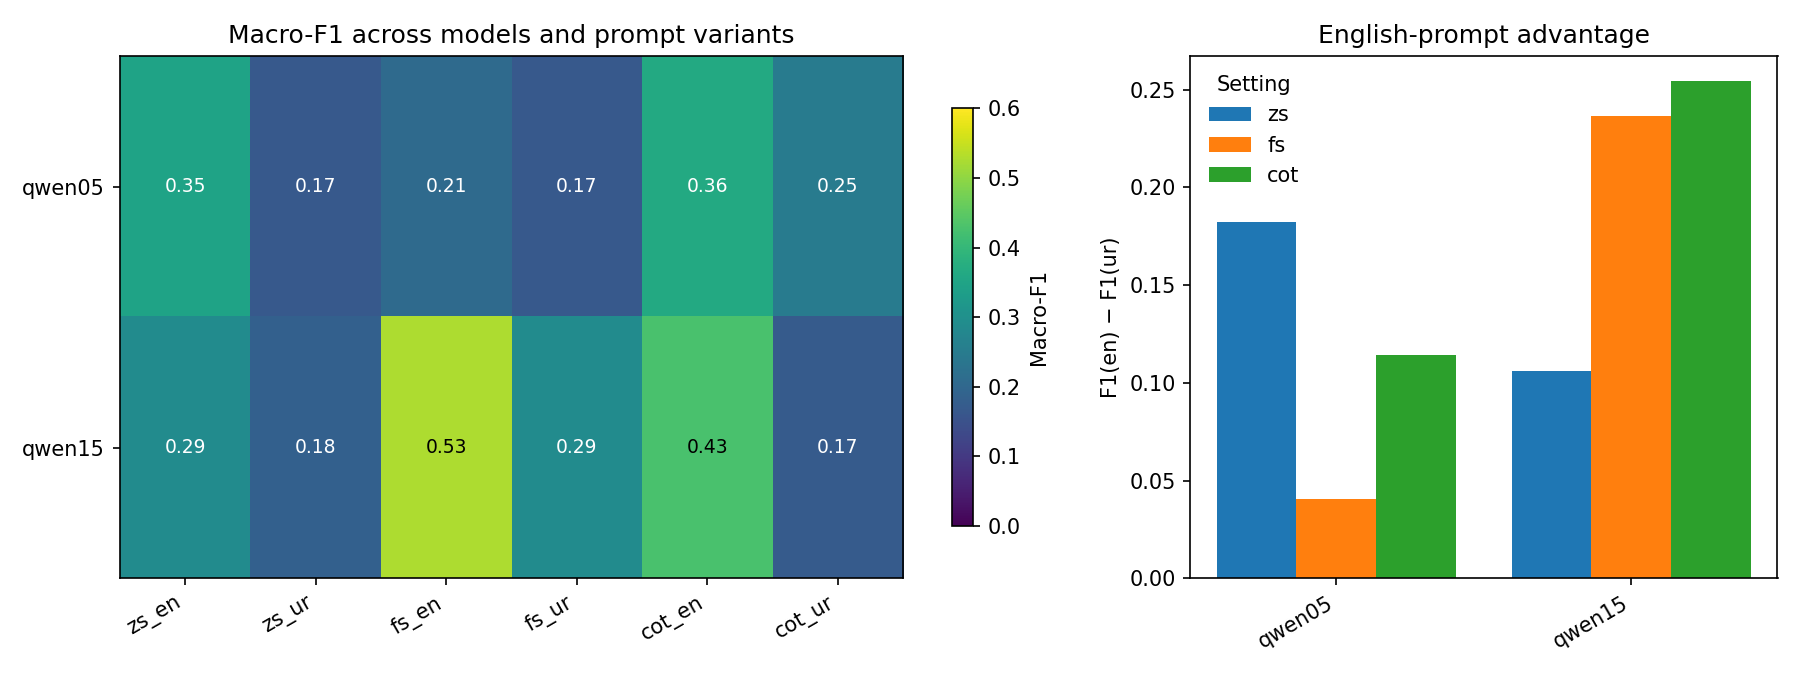
\includegraphics[width=\linewidth]{figures/heatmap_en_vs_ur.png}
\caption{Left: macro-$F_1$ for every (model, prompt) cell. Right: the
English-minus-Urdu $F_1$ advantage per model, broken down by prompting
regime. Positive bars indicate an English prompt advantage.}
\label{fig:heatmap}
\end{figure}

\subsection{Statistical significance}
Paired McNemar tests between matched English and Urdu prompts are reported
in Table~\ref{tab:sig}. Four of six pairs reach statistical significance
at $p<0.05$, all four favouring English prompts. The effect is strongest
for Qwen2.5-1.5B zero-shot ($p = 4.2\times 10^{-7}$) and few-shot
($p = 8.3\times 10^{-9}$). The two non-significant pairs are
Qwen2.5-0.5B few-shot ($p = 0.663$) and Qwen2.5-1.5B chain-of-thought
($p = 0.409$); in both cases the discordant counts ($b$ and $c$) are
close, reflecting high error rates in both the English and Urdu conditions
rather than genuine parity in classification quality.

\begin{table}[t]
\centering
\caption{Paired McNemar test between English and Urdu prompts.
$b$ = EN correct / UR wrong; $c$ = UR correct / EN wrong; $p$ = exact
binomial $p$-value. Significant results ($p<0.05$) marked with *.}
\label{tab:sig}
\begin{tabular}{llrrr}
\toprule
Model & Setting & $b$ & $c$ & $p$ \\
\midrule
Qwen2.5-0.5B & zero-shot    &  82 &  45 & $0.001$* \\
Qwen2.5-0.5B & few-shot     & 173 & 164 & $0.663$ \\
Qwen2.5-0.5B & CoT          &  85 &  41 & $<0.001$* \\
Qwen2.5-1.5B & zero-shot    &  32 &   3 & $<0.001$* \\
Qwen2.5-1.5B & few-shot     & 190 &  93 & $<0.001$* \\
Qwen2.5-1.5B & CoT          & 112 &  99 & $0.409$ \\
\bottomrule
\end{tabular}
\end{table}

% --------------------------------------------------------------------
\section{Analysis}

\subsection{Error bucketing by linguistic phenomenon}
Figure~\ref{fig:buckets} aggregates per-bucket error rates across
models for English and Urdu prompts. The buckets are computed automatically
from input text: \texttt{negation} flags Urdu/Roman negators,
\texttt{roman\_urdu\_only} flags Latin-only inputs (the entire test set),
\texttt{short}/\texttt{long} tag very brief / lengthy inputs,
\texttt{sarcasm\_like} flags exclamation-heavy inputs and common sarcastic
markers, and \texttt{refused} counts outputs that could not be parsed to
a valid label.

\begin{figure}[t]
\centering
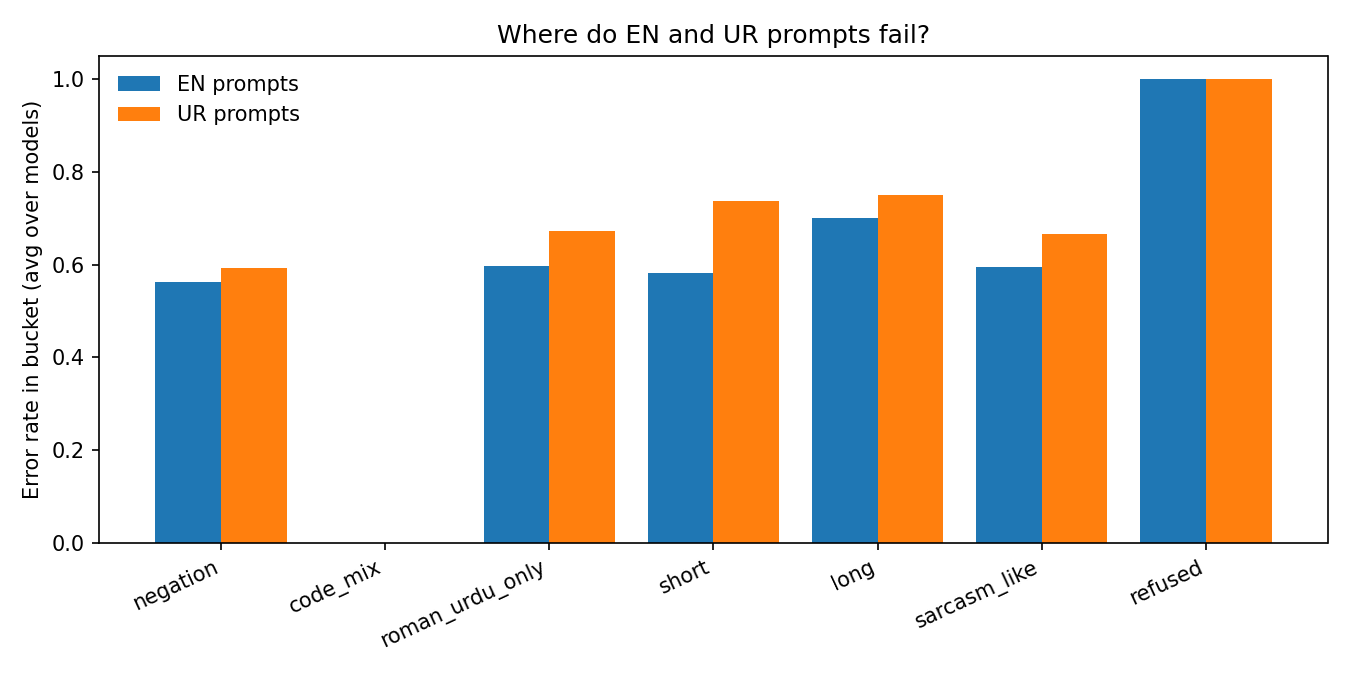
\includegraphics[width=\linewidth]{figures/per_bucket_errors.png}
\caption{Error rate per linguistic bucket, averaged over both small
LMs, separately for English and Urdu prompts.}
\label{fig:buckets}
\end{figure}

Three patterns stand out. First, the \texttt{refused} bucket is
substantially larger under Urdu chain-of-thought: Qwen2.5-0.5B
produces 115 refusals under Urdu CoT (23.1\% of the test set) versus
47 under English CoT (9.4\%), confirming that Urdu system turns impair
instruction-following when the model is asked to reason step-by-step.
Second, short inputs ($n = 117$) show the widest English--Urdu error-rate
gap: for Qwen2.5-0.5B zero-shot, the short-input error rate is 58.1\%
under English versus 79.5\% under Urdu, rising to 70.9\% vs.\ 87.2\%
under CoT; this suggests Urdu prompts strip away the contextual scaffolding
that helps short ambiguous texts. Third, negation inputs ($n = 54$) are
consistently hard regardless of prompt language, but the gap is largest
for Qwen2.5-1.5B few-shot (50.0\% EN vs.\ 77.8\% UR error rate), indicating
that few-shot demonstrations in Urdu do not reliably teach the model to
handle Roman-Urdu negation scope.

\subsection{Confusion structure}
Figure~\ref{fig:cm} shows per-cell confusion matrices.

\begin{figure}[t]
\centering
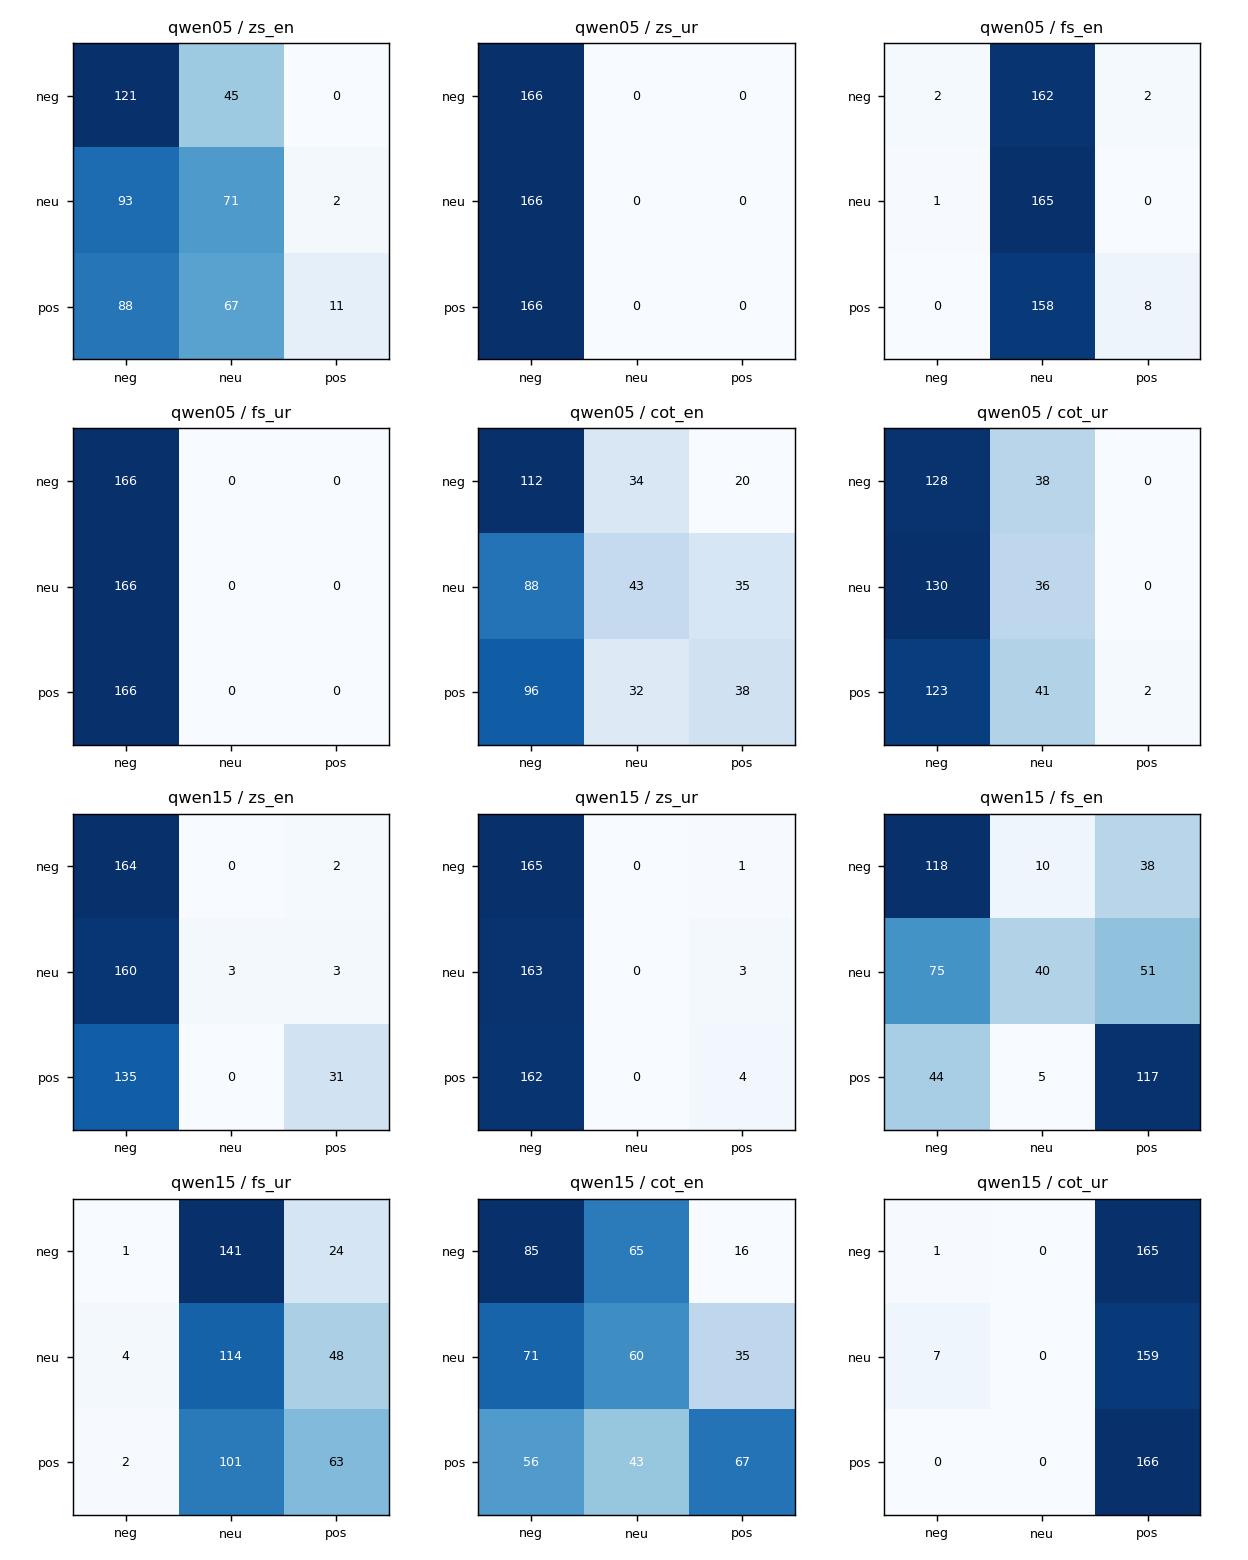
\includegraphics[width=\linewidth]{figures/confusion_matrices.png}
\caption{Confusion matrices for every (model, prompt) cell.}
\label{fig:cm}
\end{figure}

A dominant structural bias appears in Urdu-prompted cells at zero-shot
and few-shot level: both models collapse almost entirely to the negative
class. Under Qwen2.5-0.5B zero-shot Urdu, all 166 positive and all 166
neutral test examples are predicted as negative, producing macro-$F_1$
equal to the majority-class ceiling (0.167). Under Qwen2.5-1.5B Urdu
CoT the opposite collapse occurs: 165 of 166 negative examples and 159
of 166 neutral examples are predicted as positive, a label-bias pattern
consistent with \cite{zhao2021calibrate}. By contrast, the English
few-shot cell (the best-performing condition) distributes errors across
all confusion directions with no single dominant bias, suggesting that
English demonstrations convey the label space more reliably.

\subsection{Qualitative examples}
Table~\ref{tab:qual} lists representative errors from the three most
diagnostic buckets, drawn from the Qwen2.5-0.5B zero-shot condition to
isolate prompt-language effects without few-shot interference.

\begin{table}[t]
\centering
\caption{Representative errors by bucket. Translations of Roman-Urdu
inputs are given in parentheses. Predictions from Qwen2.5-0.5B zero-shot.}
\label{tab:qual}
\footnotesize
\begin{tabular}{p{0.16\linewidth}p{0.36\linewidth}p{0.07\linewidth}p{0.07\linewidth}p{0.07\linewidth}}
\toprule
Bucket & Text (Roman-Urdu, with English translation) & Gold & EN & UR \\
\midrule
negation &
  ``koi sawal nahi playstation bhot acha tha''
  ({\itshape no question, PlayStation was great}) &
  pos & neg & neg \\[4pt]
short &
  ``kitni khushi ki baat hai''
  ({\itshape what a joyous thing}) &
  pos & neu & neg \\[4pt]
sarcasm/ exclamation &
  ``NOOR PHHELA HUA AAJ KI RAAT HAI!''
  ({\itshape TONIGHT IS BATHED IN LIGHT!}) &
  pos & neg & neg \\
\bottomrule
\end{tabular}
\end{table}

The negation example illustrates a common failure: the surface token
\textit{nahi} (`not') misleads both conditions into a negative prediction
despite the overall positive sentiment. The short-text example shows a
wider gap: English zero-shot at least retrieves a non-negative prediction
(neutral), whereas Urdu zero-shot collapses to negative. All sarcasm-like
inputs carry exclamation marks or intensifiers that both prompt conditions
misread as negative.

\subsection{Discussion}
English prompts show a systematic advantage over Urdu prompts, with
statistically significant improvements in 4 of 6 paired comparisons.
The mechanism operates through two channels. At zero-shot and few-shot
levels, where both English and Urdu conditions produce no refusals, the
advantage derives from \emph{semantic instruction quality}: models
distribute their label predictions more evenly under English instructions,
while Urdu instructions trigger near-total label collapse to a single
class. This cannot be attributed to instruction-following failure
(refusal rate is 0\% for both), but rather to the model interpreting the
class semantics and decision boundary more reliably in English. At
chain-of-thought level, an additional \emph{instruction-following} channel
emerges: Qwen2.5-0.5B Urdu CoT raises refusals from 9.4\% (English) to
23.1\%, and Qwen2.5-1.5B Urdu CoT collapses to positive-only output even
with 0\% refusals---behaviour consistent with label-prior bias
\cite{zhao2021calibrate} induced when the reasoning language is outside
the model's primary instruction-tuning distribution.

Model size moderates but does not eliminate the English advantage. The
1.5B model reaches substantially higher peak performance under English
prompts (macro-$F_1 = 0.526$ vs.\ $0.364$ for 0.5B at CoT), yet the
English-minus-Urdu gap also widens with model size at the few-shot regime
($\Delta = 0.237$ for 1.5B vs.\ $0.040$ for 0.5B), suggesting that larger
models exploit English demonstrations more effectively without becoming
better at processing Urdu instructions. The most striking result is that
Qwen2.5-1.5B few-shot English (0.526) surpasses the fine-tuned
XLM-RoBERTa baseline (0.306) by a margin of 0.220 macro-$F_1$. This
result should be interpreted cautiously: the XLM-RoBERTa baseline was
trained for only three epochs on 2,000 examples without hyperparameter
search, and a more thoroughly tuned fine-tuned model would likely recover
this gap. Nevertheless, it demonstrates that lightweight prompting with
English instructions can serve as a strong starting point before fine-tuning
resources are available.

\subsection{Limitations}
This study is restricted to a single task (sentiment) and a single target
language variety (Roman-Urdu, i.e.\ Latin-script Urdu), and evaluates
only two small instruct models in the 0.5--1.5B range. The dataset inputs
are entirely Roman-Urdu, so results may not transfer to Nastaliq-script
Urdu tasks where the input script itself aligns with the Urdu prompt. Automatic error
bucketing relies on surface-level heuristics and does not capture subtle
pragmatic phenomena. Generalisation claims to other low-resource languages
or to larger model scales require additional experiments.

% --------------------------------------------------------------------
\section{Conclusion}
This paper studied whether the language of the prompt---English or
Urdu---affects the performance of small multilingual instruct LMs on Roman-Urdu
sentiment classification. Across two models, three prompting regimes, and
paired McNemar significance tests, English prompts consistently outperformed
matched Urdu prompts, with statistically significant advantages in 4 of 6
model-by-setting pairs and the largest effect at few-shot level
(macro-$F_1$ $0.526$ vs.\ $0.289$ for Qwen2.5-1.5B, $p<10^{-8}$). Error
bucketing attributes the effect primarily to two failure modes: label
collapse to a single class under Urdu zero-shot and few-shot conditions,
and elevated instruction-refusal rates under Urdu chain-of-thought---both
indicating that sub-2B models process Urdu system turns less reliably than
English ones. The practical recommendation is to prefer English instruction
prompts with Roman-Urdu input text for small instruct LMs until models in
this parameter range receive substantially more Urdu instruction-tuning
data. Future work should extend the evaluation to other low-resource
languages, to Nastaliq-script inputs, and to parameter-efficient
fine-tuning as a complement to prompting.

% --------------------------------------------------------------------
\bibliographystyle{IEEEtran}
\bibliography{references}

\end{document}
